\documentclass[11pt]{article}
\usepackage[margin=1in]{geometry}
\usepackage{amsmath,booktabs,graphicx}
\usepackage[hidelinks]{hyperref}
\emergencystretch=1em
\graphicspath{{../results/figures/}}
\title{Which Operating Conditions Are Worth Simulating?\\Value-Guided Data Acquisition for Security-Constrained Redispatch under Topology Shift}
\author{Ukachi Osisiogu\\Independent Researcher\\\href{mailto:ukachi.osi@gmail.com}{\texttt{ukachi.osi@gmail.com}}}\date{}
\begin{document}\maketitle

\begin{abstract}
Simulation labels are not equally useful when predictions feed a constrained decision. We study budgeted adaptation of a dispatch surrogate after an unseen transmission-line outage. A five-member multilayer-perceptron ensemble is trained on 220 secure-dispatch solutions from a synthetic six-bus source grid, then adapted using up to 60 labelled cases from a 160-case target pool after line 8 is removed. Random, diversity, uncertainty, and uncertainty-times-predicted-criticality acquisition are compared on the same held-out 80-case target test set across three seeds. At 60 target labels, uncertainty obtains the lowest mean dispatch error (1.387 MW) and repaired-cost regret (21.06 cost units), versus 1.425 MW and 22.42 for the decision-sensitive heuristic. All raw predictions fail an exact $10^{-7}$ MW feasibility test and require a common deterministic repair. A matched-case diagnostic shows a modest topology penalty, and rankings differ across metrics and seeds. The experiment supports decision-oriented evaluation and targeted labelling, but not the claim that the proposed operational weighting improves on uncertainty alone. Code, configurations, and results are available at \url{https://github.com/DrUkachi/value-guided-sced}.
\end{abstract}

\section{Introduction}
Security-constrained economic dispatch (SCED) maps demand and renewable availability to a low-cost generator schedule respecting network and contingency limits. Neural surrogates can approximate related optimal-power-flow mappings quickly, but feasibility generally requires explicit treatment or post-processing \cite{pan2021deepopf,fioretto2020predicting}. Topology change alters the feasible mapping, so robustness to connectivity changes is distinct from ordinary interpolation \cite{piloto2024canos}.

We ask: under an unseen line-outage topology shift and a limited target-simulation budget, which operating conditions should be labelled by a SCED oracle so that a learned surrogate reduces security violations and repaired-cost regret? Active learning commonly selects examples by uncertainty or coverage \cite{settles2009active}; decision-focused learning instead judges predictions by downstream optimization consequences \cite{wilder2019melding,mandi2022decision}. We connect these ideas using a simple acquisition heuristic that multiplies ensemble uncertainty by predicted network criticality.

Our single contribution is a leakage-controlled test of whether decision-sensitive target-case acquisition improves the operational label efficiency of a dispatch surrogate under topology shift. Four acquisition rules receive identical target-label budgets, start from identical labels within each seed, and are evaluated by prediction error, feasibility repair, and regret. The result is negative for the proposed weighting: uncertainty is strongest at the final budget on average, while predicted criticality sometimes redirects labels unhelpfully. This synthetic experiment is not evidence of deployment readiness or universal superiority.

\section{Related Work}
Learning OPF solutions replaces repeated optimization with supervised prediction. DeepOPF learns security-constrained DC-OPF dispatch and projects predictions toward feasibility \cite{pan2021deepopf}; physics-informed approaches embed equality constraints or penalize violations \cite{fioretto2020predicting}. Graph models have also targeted transfer across grid topologies \cite{piloto2024canos}. Here the architecture is fixed and the experimental variable is which target-topology simulations to purchase.

Uncertainty and representativeness are standard active-learning criteria \cite{settles2009active}. Decision-focused learning shows why predictive loss may be incomplete when predictions parameterize optimization \cite{wilder2019melding,mandi2022decision}. We use downstream quantities for evaluation but do not differentiate through SCED. Our ``decision-sensitive'' score is therefore a label-free heuristic, not a general value-of-information estimator.

\section{Problem Formulation}
An operating condition $x$ contains six-bus demands and renewable injections at buses 4 and 5. For topology $T$, the oracle returns
\begin{equation}g^*(x,T)=\arg\min_g c^\top g\end{equation}
subject to generator bounds, balance, and DC line-flow limits in the base state and after locked outages of lines 3 and 4. One preventive schedule must be feasible in all states. The source has ten lines; the target removes line 8. Acquisition observes target-pool inputs but not their labels before selection.

Given labelled source data $D_s$, initial target labels $D_t^0$, pool $U$, and batch size 12, four batches are selected. At $B\in\{12,24,36,48,60\}$ the learner trains on $D_s\cup D_t^B$ and is evaluated on a fixed target test set. The goal is operational label efficiency, not dispatch error alone.

\section{Methods and Experimental Setup}
\subsection{Oracle and data}
The linear DC-SCED oracle is solved with SciPy's HiGHS-backed optimizer. Gross demand is sampled uniformly from 140--370 MW and distributed over buses 2--6; renewable injection at buses 4 and 5 ranges from zero to 35\% of local demand. Infeasible draws are rejected. Frozen data comprise 220 labelled source cases, 160 target candidates, and 80 target test cases. Outputs include dispatch, cost, feasibility, base and contingency flows, and solve time.

\subsection{Surrogate and repair}
The ensemble contains five MLPs with two 128-unit ReLU layers, at most 300 epochs, early stopping, and source-fitted normalization. The ensemble mean is passed to a deterministic linear repair minimizing $\|g_{\rm repair}-\hat g\|_1$ subject to generator, balance, base-flow, and contingency constraints.

\subsection{Acquisition}
Random selects uniformly without replacement. Diversity uses farthest-first selection in standardized input space. Uncertainty is
\begin{equation}u(x)=\frac{1}{5}\sum_{k=1}^{5}\|\hat g_k(x)-\bar g(x)\|_2^2.\end{equation}
For decision-sensitive acquisition, target PTDFs and the ensemble mean estimate base and contingency flows. Criticality is
\begin{equation}c(x)=\max_{s,\ell}|\hat f_\ell^{(s)}(x)|/F_\ell^{\max}.\end{equation}
Both quantities are min--max normalized over the remaining pool and combined as $a(x)=\widetilde u(x)[1+\widetilde c(x)]$. Hidden candidate labels and all test data are excluded from scoring and tuning.

\subsection{Protocol and metrics}
Final seeds are 11, 22, and 33. Within each seed, methods share the initial 12 labels, architecture, retraining schedule, repair, and test cases. A raw prediction is feasible only when its balance residual and every generator, base-case line, and contingency-line violation are at most the frozen $10^{-7}$ MW tolerance. Primary outcomes are this raw-feasibility indicator and repaired regret $R(x)=C(g_{\rm repair})-C(g^*)$, measured in the synthetic linear objective's cost units. Repair magnitude is the total absolute dispatch change, $\|g_{\rm repair}-\hat g\|_1$ in MW. Dispatch MAE and individual violations are secondary. Means and 95\% Student-$t$ intervals use three seeds and are descriptive. Automated tests check split identity and leakage.

\section{Results}
\subsection{Topology shift}
On 80 matched conditions with the source-trained debugging-seed ensemble, target instead of source topology increases MAE from 1.455 to 1.531 MW, repair magnitude from 2.436 to 2.451 MW, and mean regret from 21.68 to 22.23. These modest penalties isolate transfer degradation, but seed 42 is a diagnostic rather than a three-seed estimate.

\begin{figure}[t]\centering
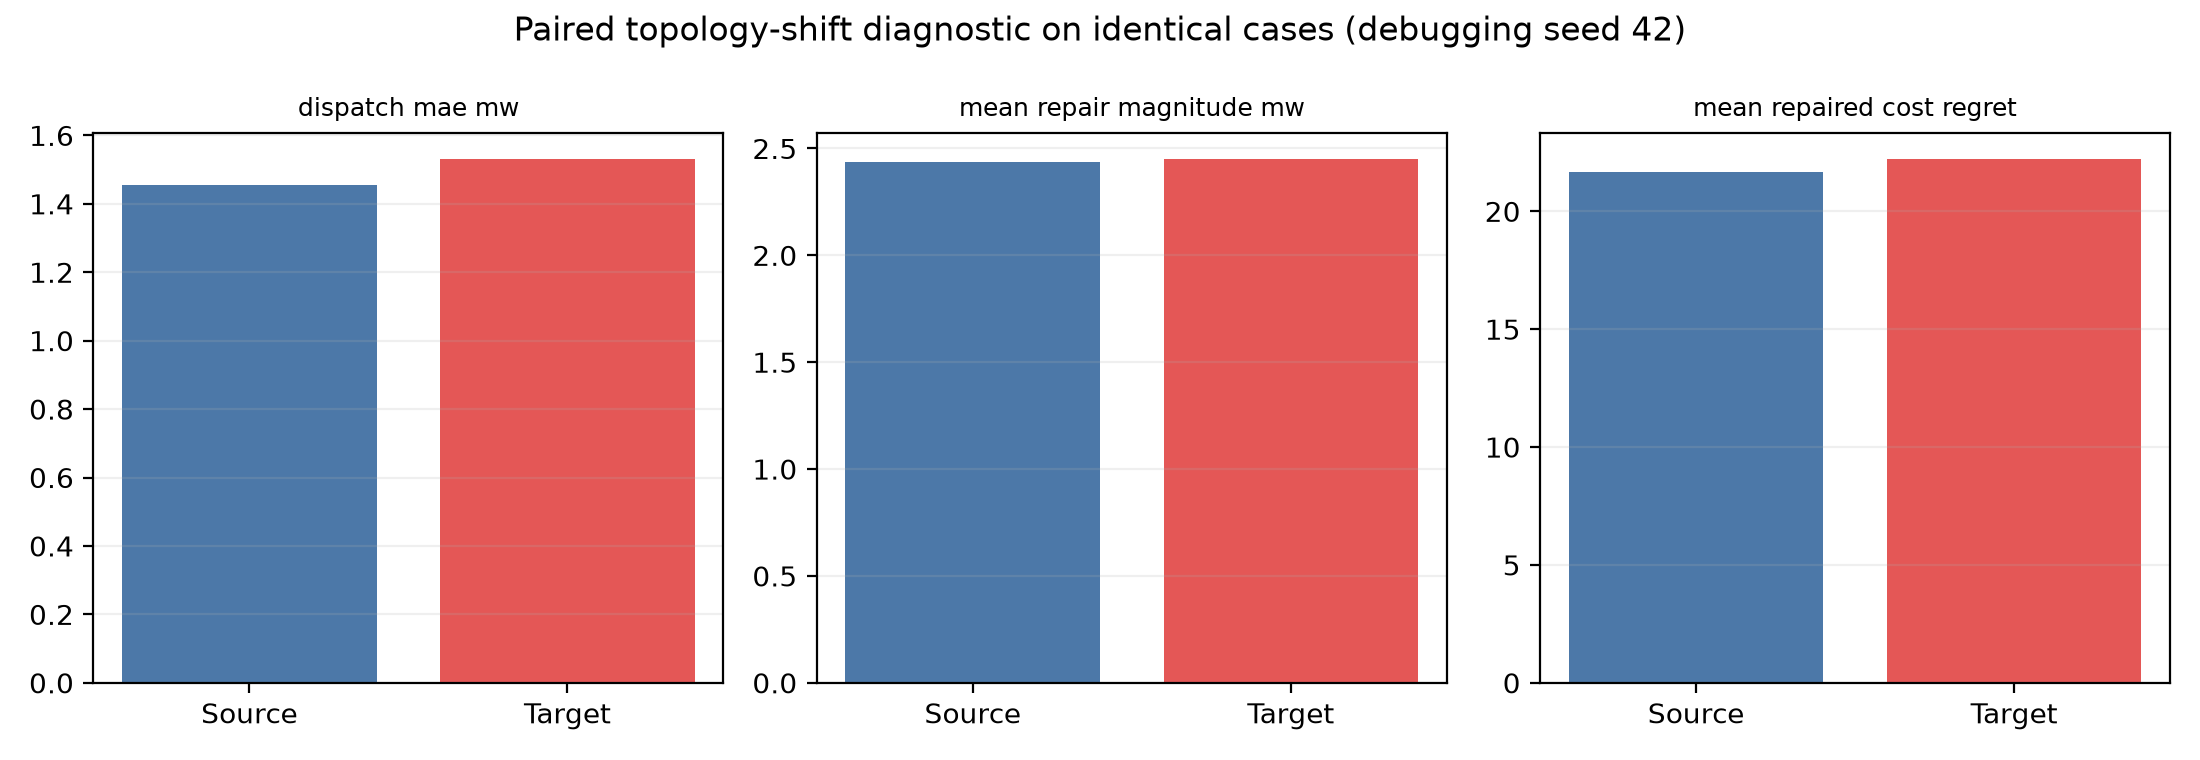
\includegraphics[width=.8\linewidth]{structural_shift_diagnostic.png}
\caption{Matched-case source-to-target topology diagnostic.}\label{fig:shift}
\end{figure}

\subsection{Label efficiency}
All methods are identical at 12 labels: mean MAE is 1.922 MW and mean regret is 28.13. At 60 labels, uncertainty has the lowest mean MAE (1.387 MW) and regret (21.06). Decision-sensitive follows at 1.425 MW and 22.42; random reaches 1.582 MW and 23.23, and diversity 1.504 MW and 23.24. Targeted selection improves average endpoints relative to random, but operational weighting does not improve uncertainty.

\begin{table}[t]\centering
\caption{Mean performance at 60 target labels across three seeds.}
\begin{tabular}{lrr}\toprule Method&MAE (MW)&Mean repaired regret\\\midrule
Random&1.582&23.23\\Diversity&1.504&23.24\\Uncertainty&\textbf{1.387}&\textbf{21.06}\\Decision-sensitive&1.425&22.42\\\bottomrule\end{tabular}
\end{table}

\begin{figure}[t]\centering
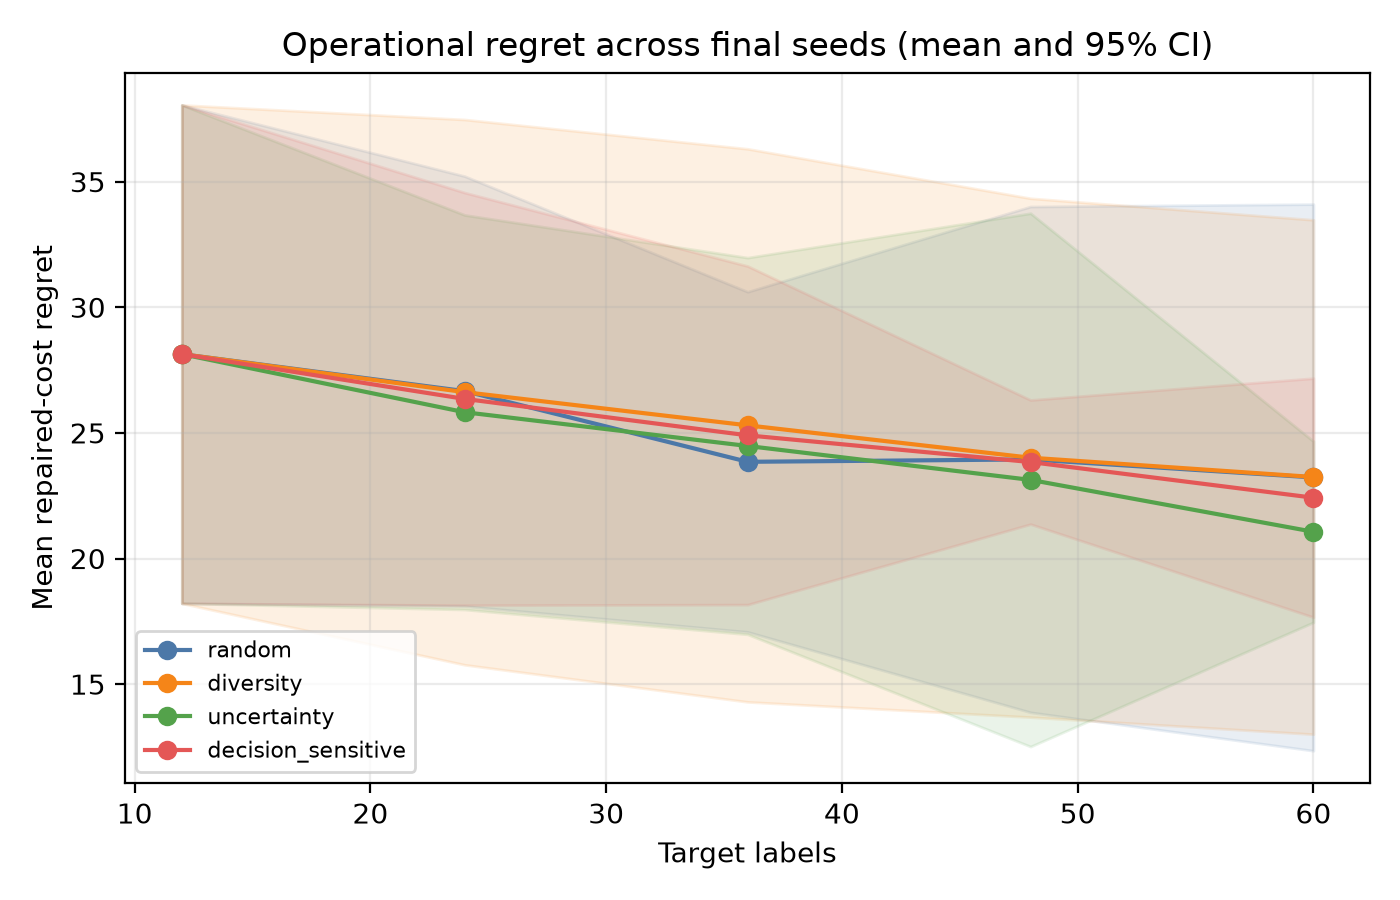
\includegraphics[width=.75\linewidth]{regret_vs_labels.png}
\caption{Mean repaired-cost regret versus target labels across three seeds; bands are 95\% $t$ intervals.}\label{fig:regret}
\end{figure}

\begin{figure}[t]\centering
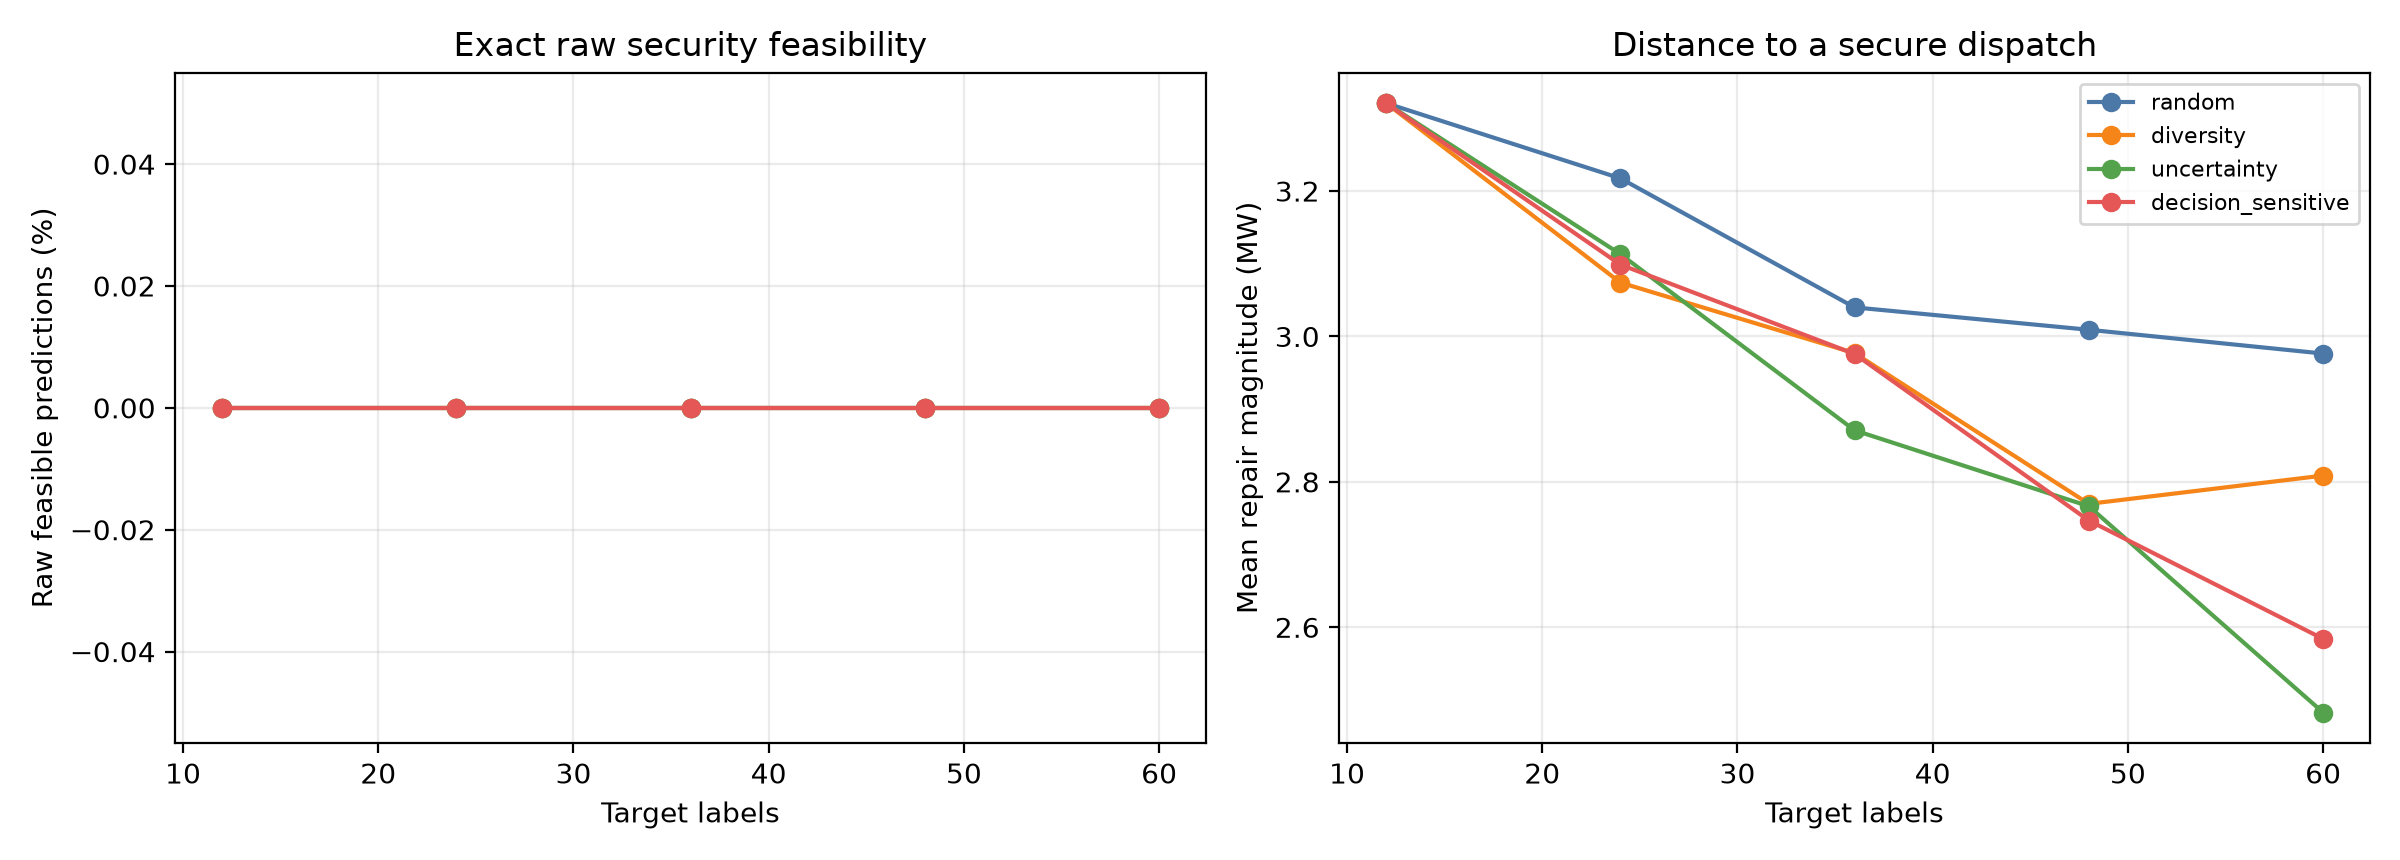
\includegraphics[width=\linewidth]{feasibility_vs_labels.png}
\caption{Left: exact raw security feasibility, which is 0\% for every method and budget. Right: mean repair magnitude (distance from the raw prediction to a secure dispatch) versus target labels.}\label{fig:feasibility}
\end{figure}

Exact raw feasibility is 0\% for every method and budget under the precommitted tolerance. This tests whether unconstrained regression directly returns a secure dispatch; it does not imply equal prediction quality. Continuous violations and repair magnitude distinguish models, while repair enables cost comparison. MAE, repair, and regret rankings differ in several seed--budget cells.

\subsection{Ablation and counterexample}
At 60 labels the combined score is worse than uncertainty by 0.038 MW MAE and 1.36 regret units. Effects vary by seed and budget. For seed 33, budget 24, test case 0045, uncertainty has zero repaired regret whereas decision-sensitive incurs 54.253, despite similar repair magnitudes (18.238 and 18.357 MW). Predicted criticality can therefore amplify model error and redirect labels unhelpfully. This rejects the frozen hypothesis that the combined heuristic is at least as useful as uncertainty alone at small budgets.

\section{Discussion and Limitations}
The result is not a universal winner: target labels help, uncertainty is a strong baseline, and a plausible operational multiplier can hurt. A risk proxy derived from imperfect dispatch inherits its errors; multiplication can compound rather than correct them. Calibration on validation data, constrained ensemble predictions, or expected repair value are future directions, not post-hoc additions to the frozen comparison.

Claims are bounded by a synthetic six-bus network, linear DC physics and costs, one target outage, two contingencies, and three seeds. The oracle is inexpensive here, so expensive simulation is motivation rather than a demonstrated bottleneck. The test set has 80 cases, exact feasibility is dominated by a stringent tolerance, and repair can conceal qualitatively different raw errors. Pool labels are precomputed but protected by code boundaries. Larger studies should test AC or dynamic simulators, multiple grids and outages, repeated dataset realizations, calibrated uncertainty, and principled value-of-information objectives.

\section{Conclusion}
Under equal SCED-label budgets, uncertainty sampling achieves the best mean final MAE and repaired regret. Adding predicted line criticality does not improve it and yields an interpretable failure case. The study supports evaluating learned dispatch through feasibility, repair, and regret while cautioning that decision-aware acquisition needs a reliable estimate of downstream value. It provides a reproducible, falsifiable foundation rather than a deployment claim.

\bibliographystyle{plain}\bibliography{references}
\end{document}
